\documentclass{beamer}
\usepackage[T1]{fontenc}
\usepackage{lmodern}

\mode<presentation>
\usetheme[footline=empty]{Magicc}

\usepackage{graphicx}
\graphicspath{{figures/}}
\DeclareGraphicsExtensions{.pdf, .png, .jpg}

\usepackage{tikz}

% add logo to slide header
\addtobeamertemplate{frametitle}{}{%
\begin{tikzpicture}[remember picture,overlay]
\node[anchor=north east,yshift=2pt] at (current page.north east) {
\includegraphics[height=0.75cm]{logo_white}};
\end{tikzpicture}}

% create outline slide at each \section{} (optional)
\AtBeginSection[]{\frame{\frametitle{Outline}\tableofcontents[currentsection]}}

% presentation info
\title{Multi-dimensional Optimization of Gasoline-fueled Variable Pitch Multirotor Aircraft}
%\title[Short Title]{GAS Quad}
\author{Dallin Briggs, Gary Ellingson}
\institute[MAGICC Lab]{
\includegraphics[height=0.5in]{logo_gray}}
\date{\today}

\begin{document}

\begin{frame}
\titlepage
\end{frame}


\begin{frame}{Introduction}

	What is a gas multirotor?
	\begin{itemize}
	\item{Uses a single small two-stroke engine.}
	\item{Power is transfered through torque tubes to the rotors.}
	\item{All rotors must be variable pitch.}
	\item{Theoretically capable of longer flight times than battery powered multirotors because of higher specific energy of gasoline.}
	\item{FAA requires less then 55lbs}
	\end{itemize}
\end{frame}

\begin{frame}{Motivation and Background}
	\begin{center}
	Currently available multirotor capabilities
	\end{center}
	\begin{figure}
		\begin{center}
			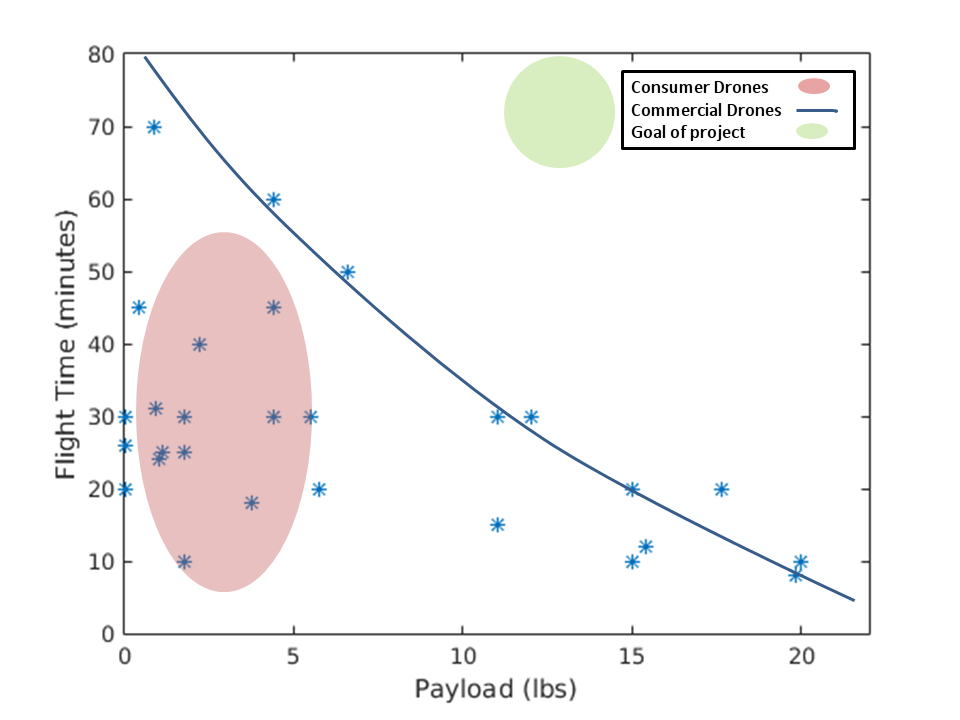
\includegraphics[width=.70\textwidth]{../current_capabilities.png}
			\label{current_capabilities}
		\end{center}
	\end{figure}
\end{frame}

\begin{frame}{Engine Models}

	\begin{figure}
		\begin{center}
			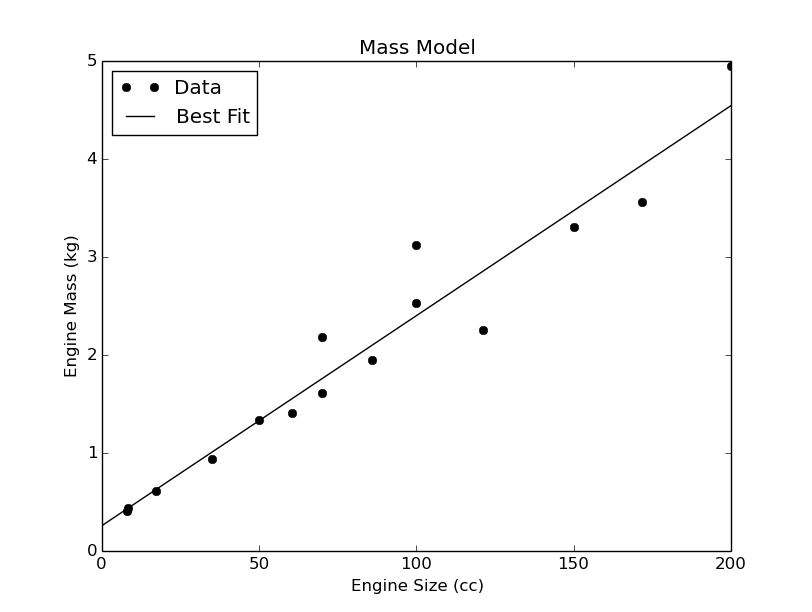
\includegraphics[width=.70\textwidth]{../mass.png}
			\label{fig:eng_mass}
		\end{center}
	\end{figure}
\end{frame}

\begin{frame}{Engine Models}	
	\begin{figure}
		\begin{center}
			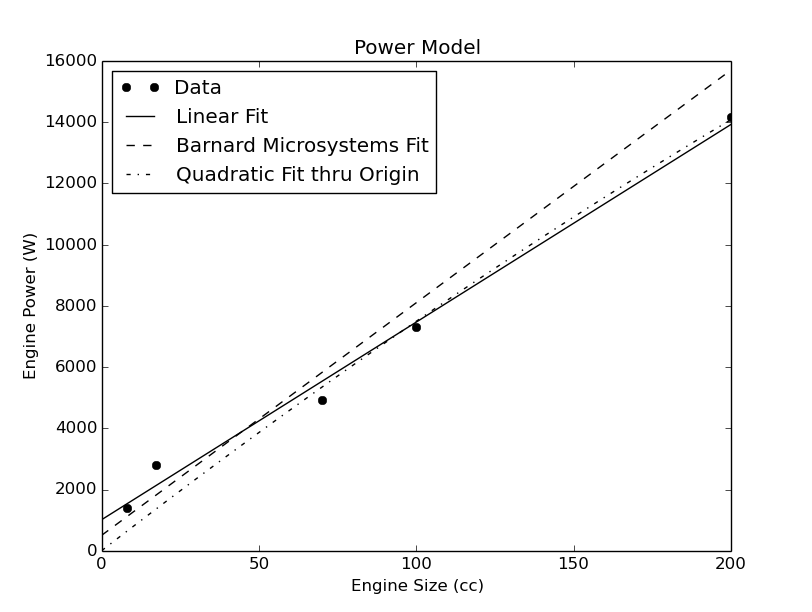
\includegraphics[width=.70\textwidth]{../max_power.png}
			\label{fig:eng_power}
		\end{center}
	\end{figure}
	
\end{frame}

\begin{frame}{Aerodynamic Model}
	\begin{itemize}
		\item{To represent the aerodynamics of each rotor, we used Combined Differential Blade Element and Momentum Theory for nonuniform inflow.}
		\begin{center}
		$$ dT = \frac{1}{2} \rho a \Omega^2 r^2 (\theta - \phi) c \  dr $$
		$$ dQ = \frac{1}{2} \rho \Omega^2 r^3 c (\delta + \phi C_L) \ dr $$
		\end{center}
	\end{itemize}

\end{frame}

\begin{frame}{Optimization Method}
	Design Variables
	\begin{itemize}
		\item{Engine Size}
		\item{Rotor Size}
		\item{Fuel Capacity}
		\item{Fuel Burn Rate}
		\item{Rotor Pitch Angle}
		\item{Head Speed}
	\end{itemize}
	
	$Flight Time = f(Fuel Capacity, Fuel Rate)$
	
	$C: P_{Shaft} \geq P_{Rotor}, T \geq W_{total}, P_{max} \geq P_{Shaft}, 55lbs \geq W_{total} $ 
	
	SNOPT to optimize

\end{frame}

\begin{frame}{Results}
	\begin{figure}
		\begin{center}
			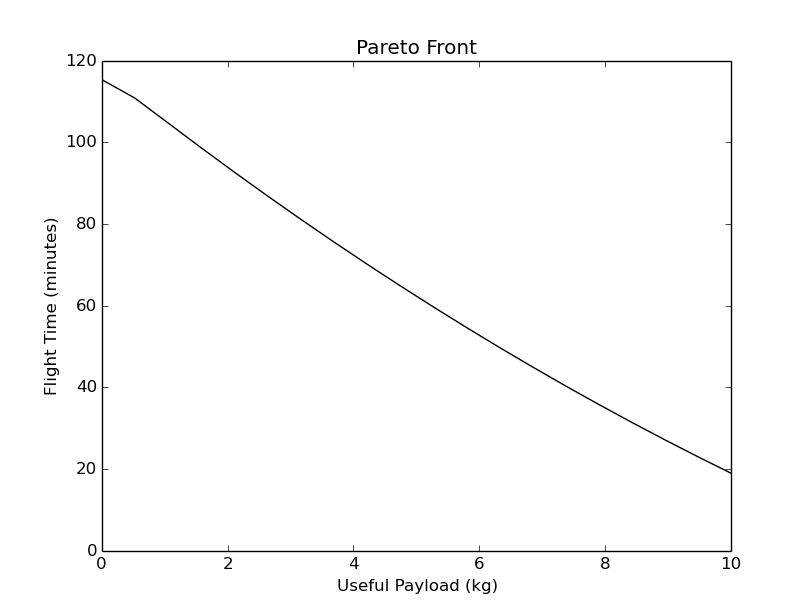
\includegraphics[width=.70\textwidth]{../pareto_front.png}
			\label{fig:pareto}
		\end{center}
	\end{figure}
\end{frame}

\begin{frame}{Results}
	\begin{figure}
		\begin{center}
			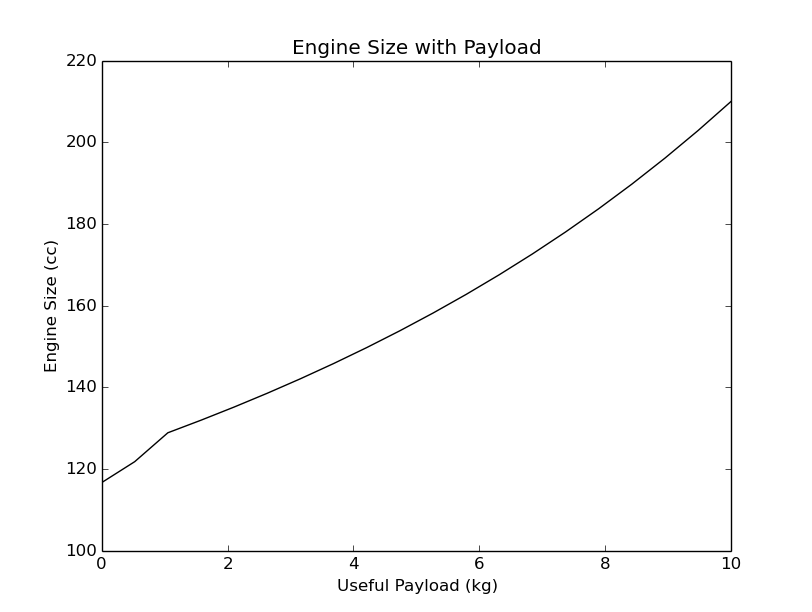
\includegraphics[width=.70\textwidth]{../engine_size_vs_payload.png}
			\label{fig:pareto}
		\end{center}
	\end{figure}
\end{frame}

\begin{frame}{Results}
	Simultaneously optimize over 3, 5, and 7 kg payload
	\begin{itemize}
		\item{Engine Size: 177 cc} 
		\item{Rotor Size: 2.16 m}
		\item{Fuel Capacity: 6.45 kg}
		\item{Fuel Burn Rate: 0.0019 kg/s}
		\item{Rotor Pitch Angle: 17.618 deg}
		\item{Head Speed: 135.09 rpm}
	\end{itemize}
	
	Flight Time > 42.47 minutes
	
	Payload < 7 kg
\end{frame}

\begin{frame}{Lessons Learned}
	\begin{itemize}
		\item{Large, Slow props - https://youtu.be/syJq10EQkog?t=7s}
		\item{Helicopter rotor dynamics are difficult to conceptualize and calculate.}
		\item{Over-simplification of aerodynamic model leads to unrealistic results.}
		\item{Scaling the problem was critical}	
	\end{itemize}
\end{frame}

\begin{frame}{Questions}
	
		\begin{center}
			Questions?
		\end{center}
	
\end{frame}

\end{document}

